\begin{figure}[!htb]
    \centering
    \caption{\textbf{Impact of Noise on Mean Wealth Distribution} \\ 
    \small{
    The figure shows the distribution of the estimated parameters when we add a random number from a normal distribution with mean 0 and standard deviation 0.1 to the mean wealth. We re-estimate the model using the new moments for 1000 times and compare the results with the original estimates.  The green line represents the original estimates. The red line represents the estimates when we add noise to the mean wealth. The blue line represents the estimates for different values of the mean wealth. The red dashed lines represent the 5th and 95th percentiles of the distribution of the estimated parameters. The black dashed line represents the true value of the moment.
    We report the results for $\beta$ in (a), $\gamma$ in (b), and $\phi$ in (c).
    }
    }
    \label{fig:robustness_check}

    \subfloat[][Robustness Check for $\beta$]{
    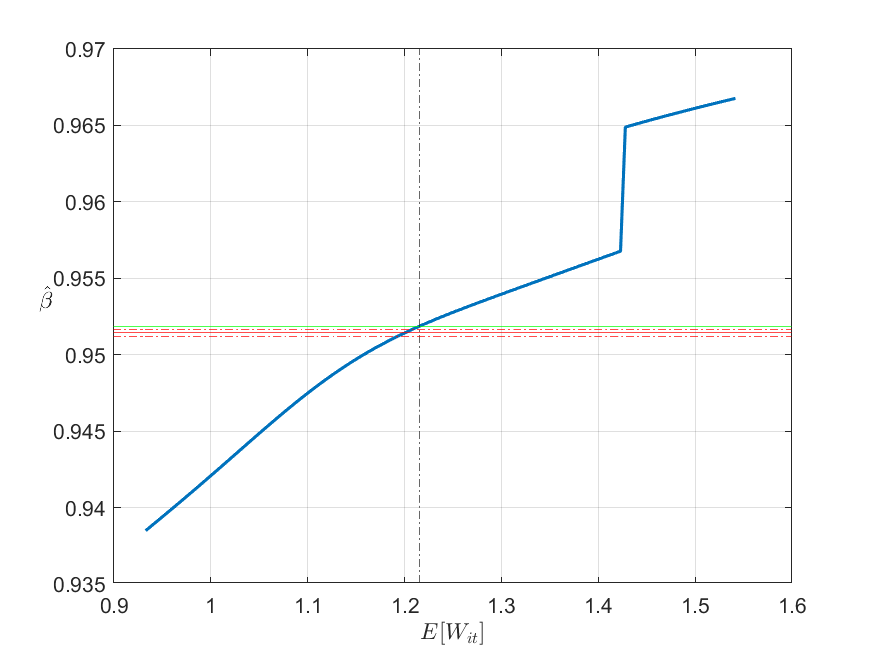
\includegraphics[width=0.45\linewidth]{Figures/robustness_check_parameterbeta.png}
    }   
    \subfloat[][Robustness Check for $\gamma$]{
    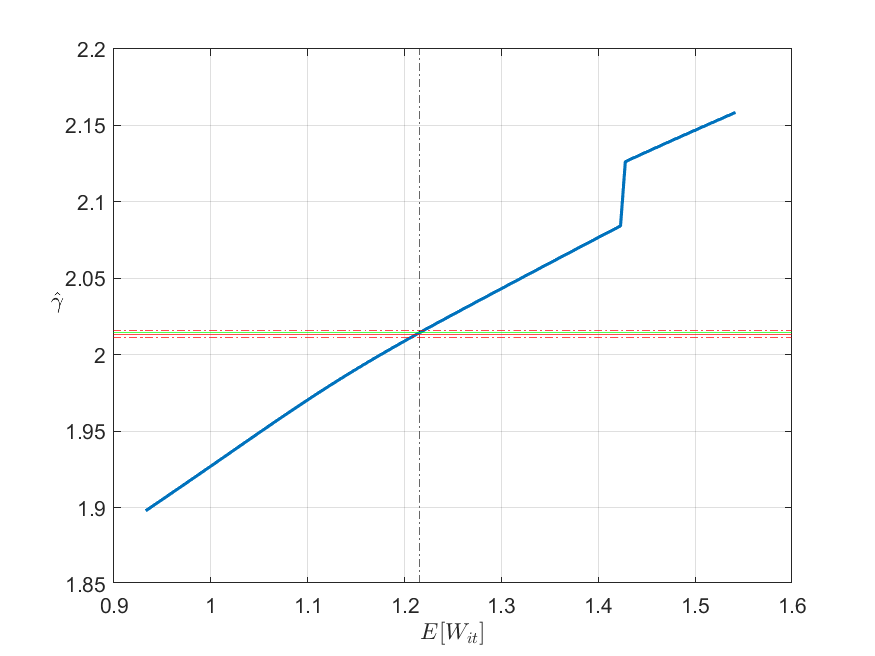
\includegraphics[width=0.45\linewidth]{Figures/robustness_check_parametergamma.png}
    }\\
    \subfloat[][Robustness Check for $\phi$]{
    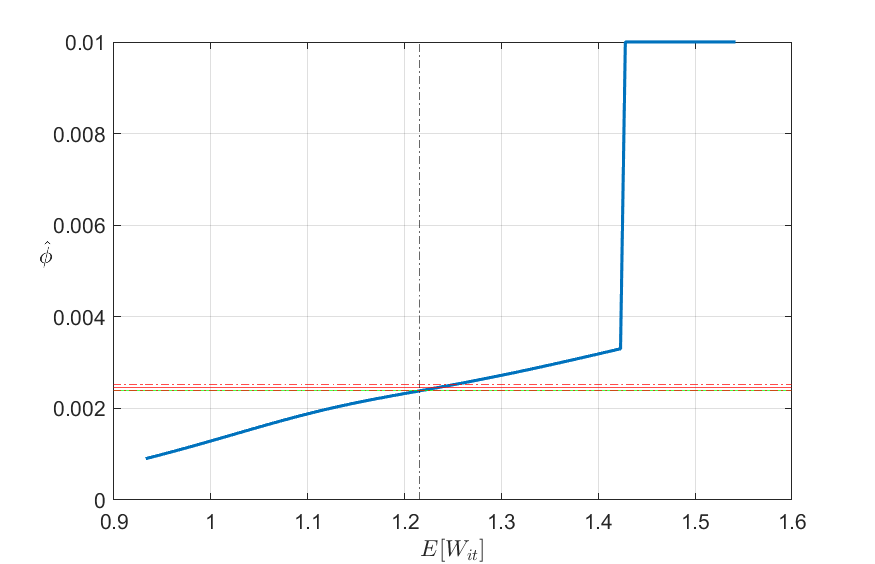
\includegraphics[width=0.45\linewidth]{Figures/robustness_check_parameterphi.png}
    }
\end{figure}